\chapter{Background}
\label{chap:background}
In order to grant a better understanding of the subsequent chapters, this chapter is going to provide a background to the terms and concepts used in the thesis\dots

\section{Remote Direct Memory Access (RDMA)}
\label{sec:RDMA}
\ac{RDMA} is an alternative to the traditional \ac{TCP/IP} network communication protocols. In short, \ac{RDMA} can provide access to a remote machine's memory without performing unnecessary intermediate copies of the memory while also bypassing the CPU of the remote machine.\\
RDMA has been gaining traction in the academic community (Figure \ref{fig:rdmaHits}). This growing popularity is because \ac{RDMA} overcomes some limitations by \ac{TCP/IP}, and by doing so, helps to provide high bandwidth and low latency.
Therefore, in order to explain \ac{RDMA}, the shortcomings of \ac{TCP/IP} socket programming is stated, and thus motivating the benefit of \ac{RDMA}.

\begin{figure}[h]
  \centering
  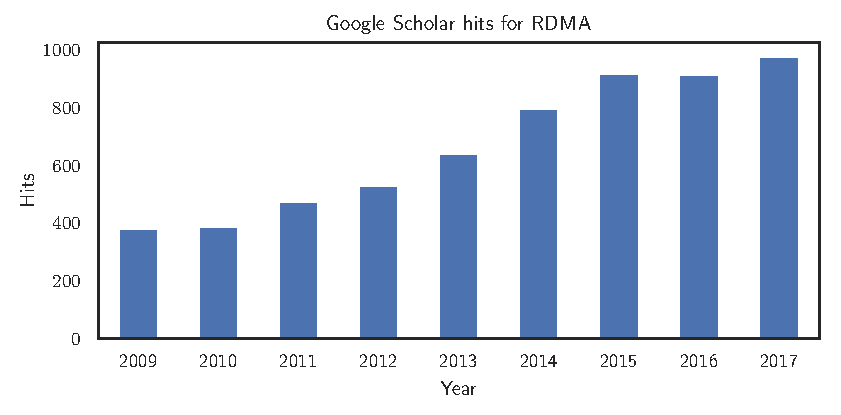
\includegraphics[width=0.7\linewidth]{GoogleScholarRDMAHits.pdf}
  \caption{Google Scholar hits of RDMA keyword}
  \label{fig:rdmaHits}
\end{figure}